\section{Implementation}

\subsection{UDS implementation of the Scapy library}

\begin{samepage}
    \begin{minted}{python}
    class UDS(ISOTP):
        services = {
             0x10: 'DiagnosticSessionControl',
             # [...]
             0x22: 'ReadDataByIdentifier',
             # [...]
             0x7f: 'NegativeResponse'})
        fields_desc = [
            XByteEnumField('service', 0, services)
        ]
    \end{minted}
\end{samepage}
    
%TODO: Why inherting from ISOTP

The UDS class contains only the service field. Even though the whole UDS protocol is in the application layer, the Scapy implementation starts a new class whenever the subsequent fields depend on one field of the current layer. This is the case here, since the next fields depend on the value of the service field. The service specific fields are defined in their own classes, for example:

\begin{samepage}
\begin{minted}{python}
class UDS_DSC(Packet):
    diagnosticSessionTypes = { ... }
    fields_desc = [
        ByteEnumField('diagnosticSessionType', 0,  diagnosticSessionTypes)
    ]
\end{minted}
\end{samepage}

A UDS packet enabling the extended diagnostic session would be created with:

\begin{samepage}
\begin{minted}{python}
packet = UDS() / UDS_DSC(diagnosticSessionType='extendedDiagnosticSession')
\end{minted}
\end{samepage}

UDS not only allows to read data, but also to write. Which makes it especially critical for security. For example the firmware of an ECU can be updated through this protocol. This usually requires higher privileges, which can be gained through the previously mentioned SecurityAccess service.

\subsubsection{How to work with the ISO-TP protocol}

The can-utils tools also contain applications to handle ISO-TP communication. Since this is never used in this work, but the Scapy implementation is, only the Scapy implementation is explained.

As for the CAN implementation, there are two ISO-TP socket implementations in Scapy. A software and a native implementation. Until including Linux kernel 5.9, the corresponding ISO-TP module for Linux had to be installed separately \cite{isotp-module}. Since Linux kernel 5.10, it is part of the Linux mainline kernel \cite{isotp-commit}. Both implementations handle the ISO-TP metadata themselves, i.e.  fragmentation, defragmentation, etc.

An ISO-TP socket contains a source and destination identifier. They offer the same functionality as the ports for TCP or UDP. The source identifier is the identifier of outgoing CAN packets, and the destination identifier is the identifier expected for incoming packets.

The usage of the native implementation is illustrated in the following code snippet:

\begin{samepage}
\begin{minted}{python}
from scapy.contrib.isotp import ISOTPNativeSocket
socket = ISOTPNativeSocket('vcan0', sid=0x123, did=0x456)
packet = Raw(b'\x01\x02')
socket.send(packet)
\end{minted}
\end{samepage}

\subsection{Explaining the service enumerators of the UDS Scanner}

% TODO: Add that it was still work in progress while doing this work
% and thus, that problems occured and had to be fixed.
% Out of scope of this work.

Enumerators are service-specific and create all possible requests for a service.
For example, the enumerator for the DSC service is called UDS\_DSCEnumerator. The most important member of the enumerator classes is the \mintinline{python}{_get_initial_requests} method. The return value is an iterable object which contains all requests for this service. DSC has an eight bit identifier, leading to a maximum of 2\textsuperscript{8} packets for this service. Each enumerator will be executed for each found state of the ECU. So, if an enumerator already ran, and afterwards a new state is found, this enumerator will run again within the same scan with the new-found state.

For a better understanding, the UDS\_DSCEnumerator implementation will be described exemplary.

\begin{samepage}
\begin{minted}{python}
class UDS_DSCEnumerator(UDS_Enumerator, StateGenerator):
    def _get_initial_requests(self, **kwargs):
        session_range = kwargs.pop('session_range', range(2, 0x100))
        return UDS() / UDS_DSC(diagnosticSessionType=session_range)
\end{minted}
\end{samepage}

The method can be given keyword parameters. The only one used here is \mintinline{python}{session_range}. If none is given, which is usually the case, it defaults to the range from 0x02 to 0xff. So, this enumerator creates 254 packets for each state. This service is a StateGenerator, which means its requests can change the state of the ECU. This is detected by the UDS Scanner and the new state will be scanned as well.

So-called staged enumerators contain enumerators where each enumerator is a stage. They start executing the first enumerator for each state, followed by each subsequent enumerator in the same way. For each stage transition (for example $1 \rightarrow 2$ or $2 \rightarrow 3$) connectors can be defined. They are functions with two arguments, containing the previous enumerator and the new enumerator. Here the results of the previous enumerator can be evaluated and the new enumerator can be configured accordingly.

Enumerators can output their results as a text-table. For example:

\begin{samepage}
\begin{minted}{text}
---------------+---------------+---------------+---------------+
               | session1      | session1tp1   | session3tp1   | 
---------------+---------------+---------------+---------------+
TesterPresent: | PR: Supported | PR: Supported | PR: Supported | 
---------------+---------------+---------------+---------------+
\end{minted}
\end{samepage}

This means, the request of the TesterPresent service was positively answered by the ECU in all three found states.

\subsection{Implementing new enumerators for the RC service}

Three classes are of interest:

\begin{itemize}
    \item \textbf{RCEnumerator}: Defaults to scanning the whole RC service, including all three types.
    \item \textbf{RCStartEnumerator}: Only scanning Type1 of the RC service.
    \item \textbf{RCSelectiveEnumerator}: Staged enumerator containing an RCStartEnumerator and an RCEnumerator.
\end{itemize}

\begin{figure}[h]
    \centering
    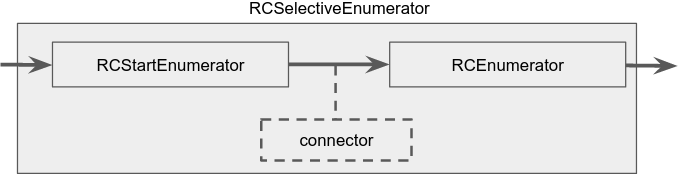
\includegraphics[width=0.7\textwidth]{rc-schematic}
    \caption{Schematic illustration of the new RCSelectiveEnumerator.}
    \label{fig:rc-schematic}
\end{figure}

The connector of the RCSelectiveEnumerator expands the found identifiers of the RCStartEnumerator to ranges and also resolves any overlaps to a continuous range and forwards these ranges to the second stage, the RCEnumerator. Additionally, the connector configures the RCEnumerator to only scan Type2 and Type3.

Each positively answered identifier of Type1 in any state will also be probed for all subsequent states in Type2 and Type3, even if this identifier is not found in Type1 for another state. This increases the coverage in cases, where a routine can be started in a state, but its result, or to stop it, may only be requested in another state.

The full implementation can be seen in \autoref{app:rc-implementation}.

\subsection{Implementing new enumerators for the RDBI service}

Again, three classes are of interest:

\begin{itemize}
    \item \textbf{RDBIEnumerator}: Defaults to scanning the whole RDBI service.
    \item \textbf{RDBIRandomEnumerator}: Scanning block-based with random identifiers.
    \item \textbf{RDBISelectiveEnumerator}: Staged enumerator containing an RDBIRandomEnumerator and an RDBIEnumerator.
\end{itemize}

\begin{figure}[h]
    \centering
    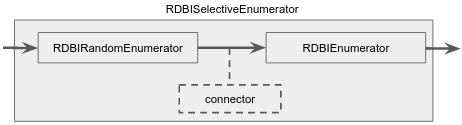
\includegraphics[width=0.7\textwidth]{rdbi-schematic}
    \caption{Schematic illustration of the new RDBISelectiveEnumerator.}
    \label{fig:rdbi-schematic}
\end{figure}

Similar to the previous approach, the new implementation is two-staged. First, the RDBIRandomEnumerator is executed. Then, the connector creates requests for whole blocks, if any of their requests were answered positively, and ensured that for a single block each identifier is queried only once. The resulting packets are passed to the configurable RDBIEnumerator.

Also, as with the RCSelectiveEnumerator, each positively answered identifier will be remembered for all subsequent states. This increases the coverage because most identifiers are also available in other states, but the RandomEnumerator might not detect them for each state.

Implementing the RDBIRandomEnumerator was a challenge because it must include the probabilities of occurence of positively responded identifiers for each block. With a block size of $2^6$, there would need to be a list with $\frac{2^{16}}{2^6} = 1024$ elements. Thus, it is desirable to represent this information more compactly. A better representation is based on two facts. That the probabilities are ultimately calculated to the number of samples, and that at least one request should be generated for each block. For the former, the number of samples for each block were pre-computed instead of being computed at runtime. This simplifies the list in the sense that integers are stored instead of float values. Second, the number of samples is not stored for all blocks, but only for blocks whose number of samples is greater than or equal to 2. And blocks for which no value is stored, the value 1 is used. This automatically solves that each block is probed with at least one packet, even if its probability is 0\%. These simplifications transformed the list of 1024 elements into a dictionary of only 109 elements.

The non-compact version is shown in \autoref{app:random-not-compact} and the final implementation in \autoref{app:rdbi-implementation}.

\subsection{Extending the UDS Scanner to skip unsupported services}

In contrast to the previous approaches, this one is not applied to an enumerator, but to the UDS Scanner itself. The UDS Scanner evaluates each response, for example to detect if a new state was found. Here, a check was added for negative responses if they have the NRC 0x11 or 0x7f. If they do, the enumerator is set to completed for the currently executed state. This behavior has to be enabled explicitly, because as the next section explains, it might result in losses.
